\documentclass[a4paper, 10pt]{article}

\usepackage[margin=1.0in]{geometry}
\usepackage{mathtools}
\usepackage{amssymb}
\usepackage{graphicx}
\usepackage{hyperref}
\usepackage{physics}
\usepackage{hanging}

\begin{document}

\title{Public-key criptography and the issues it faces with the emergence of quantum computers}
\author{Marko Vejnovi\'{c}}
\maketitle

\section{Rationale}
\subsection*{}
\paragraph*{}
As someone who is interested in computers, criptography has always piqued my interests. Although we use some sort of 
encryption almost every time we access the internet, my first interaction with cryptographic algorithms was when using 
the \textit{SSH} protocol.\footnote{The Secure Shell (SSH) Protocol is a protocol for secure remote login and other
secure network services over an insecure network (Internet Requests for Comments, 2006).} The \textit{OpenSSH}
implementation can be configured to use different encryption algorithms, out which I found \textit{RSA}
\footnote{Rivest-Shamir-Adleman} to be the most interesting one, as it is by far the most commonly used one. Exploring
this algorithm sparked interest in me to further explore the field of cryptography, especially modern cryptography.

\section{Introduction}
\paragraph*{}
\textit{Cryptography} is the study of confidential communications in the presence of adversaries (Leeuwen, J. van.). 
The process of converting a readable message\footnote{Refered to as \textit{plaintext} or \textit{cleartext}} into an 
undiscernable message\footnote{Refered to as ciphertext} is called \textit{enciphering}, whereas the process of 
converting an enciphered message into readable form is refered to as \textit{deciphering} (ISO 7498-2:1989). The 
mathematical function which is used for enciphering and deciphering is called a \textit{cipher} (Schneier, Bruce). 
Usually these operations require different functions. A message $M$ is enciphered using the function $E$ to a 
ciphertext $C$.
$$E(M) = C$$
This ciphertext is then deciphered using $D$ back into $M$ again.
$$D(C) = M$$
Cryptography requires that the following is true, as the essence of ciphers is being able to recover the original
plaintext (Schneier, Bruce):
$$D(E(M)) = M$$

\paragraph*{}
It is worth noting that characters, symbols or other similar notions are represented with numbers in the majority of 
cryptogrpahic systems.

\paragraph*{}
Historically, two types of ciphers existed - \textit{restricted ciphers} and \textit{key ciphers}. The former relied 
on adversaries not knowing the cipher itself. The earliest of ciphers, such as the \textit{Atba\v{s} cipher} were, 
indeed, restricted ciphers. Restricted ciphers have almost completely vanished from use, as they present many issues - 
no quality control, no standardization and modern computers being able to crack such types of ciphers only being a few 
of them (Schneier, Bruce). Key ciphers present themselves as a solution to these issues. Both enciphering and 
deciphering is done using a key:
$$E_k(M) = E(M, k) = C$$
$$D_k(C) = D(C, k) = M$$

\paragraph*{}
For the majority of the history of cryptography, \textit{symmetric ciphers} were employed. Symmetric ciphers are 
ciphers where the same key for enciphering and deciphering must be used.
$$E_k(M) = C$$
$$a \neq k \implies D_k(C) \neq M$$

\paragraph*{}
One of the first notable uses of a symmetric key cipher was the \textit{Caesar's cipher}. It, among other substitution 
ciphers, shifted a character in the alphabet to another by the key $k$, in an alphabet which has $N$ characters:
$$C = M + k \mod N$$
$$M = C - k \mod N$$

Other similar, more complex, systems have emerged throughout history.

\subsection{Modern cryptography}
\paragraph*{}
Until 1976, with the publication of ``\textit{New Directions in Cryptography}'' by Whitfield Diffie and Martin E. 
Hellman\footnote{Actually, this paper was preceeded by James Ellis's work (1975), however, Ellis's work remained top 
secret in the \textit{Goverment Communications Headquarters} until 1997, when it was fully released to the public 
(Sawer, Patrick).}, the key was necessary to be transmitted in secrecy. The work of this paper resulted in an algorithm
 which allowed for transmitting a key in public, called the \textit{Diffie-Hellman key exchange}. 
``\textit{New Directions in Cryptography}'' is the paper with which modern cryptography starts.

\paragraph*{}
The Diffie-Hellman key exchange does however, have two issues. The first is that there is a need for a courier to 
actually transmit the key (although the courier does not know what the key is). The second issue is that the listening 
party has no way of knowing if a message received was sent by the expected party.

\paragraph*{}
\textit{Public-key ciphers} present themselves as a solution to both of these issues. Public-key ciphers are ciphers 
which operate by using different keys for enciphering and deciphering.
\begin{equation} \label{pk-encipher}
C = E_{k1}(M)
\end{equation}
\begin{equation} \label{pk-decipher}
M = D_{k2}(C)
\end{equation}
These ciphers are called ``\textit{public-key}'' because the enciphering can be done in public. The enciphering key is 
called the \textit{public key}, whereas, the deciphering key is denoted to as the \textit{private key}. Anyone is able 
to enipher a message using the public key, but only specific people are able to decipher it with their private key. The
 most widely known, and most widely used public-key cipher is the \textit{RSA}\footnote{Rivest-Shamir-Adleman} 
cipher\footnote{The paper ``\textit{A Method For Obtaining Digital Signatures And Public-Key Cryptosystems}'' was published
 by Rivest, R. L. et al. in 1977.}.

\paragraph*{}
Both of these ciphers are based on modular arithmetic. For analyzing how well different algorithms perform, the notion 
of \textit{time complexity} is used\footnote{Time complexity is a measure of the time taken to perform a certain 
algorithm in terms of individual instructions. It is the number of instructions required $O(n)$ to perform on input 
whose size is $n$. To exemplify, a function which searches for an element in an array of length $n$ takes $n$ 
instructions to perform - for every element of the array, a check is done to see whether the element is the one that is
 searched for.}.

\section{Modular arithmetic}

\subsection{Introduction}
\paragraph*{}
It was Gauss who gave the modern definition of modular arithmetic: If a number $m$ divides the difference of the 
integers $b$ and $c$\footnote{These integers can be positive or negative, they are taken absolutely, unsigned.}, 
$b$ and $c$ are \textit{congruent relative} to $m$, otherwise, they are \textit{noncongruent}. The number $m$ is 
defined as the \textit{modulus} (Gauss, Carl Friedrich). If the numbers $b$ and $c$ are, indeed, congruent, they are 
called a \textit{residue} of the other.

\paragraph*{}
For a number $a$, all of its residues modulo $m$ are contained in the formula
$$a + km$$
where k is any integer (Gauss, Carl Friedrich).

\paragraph*{}
Gauss also introduced the modern congruence notation\footnote{It is worth noting that Gauss in reality wrote the 
modulus in parenthesees $$a \equiv b \pmod{m}$$ but for the purposes of this paper, I will use the more modern, also 
widely accepted, parenthesees-less notation.}:
$$a \equiv b \mod m$$

\paragraph*{}
To exemplify the previous statements:
$$5 \equiv 28 \mod 23$$
$5$ is congruent to $28$ modulo $23$ means the following:
\begin{gather*}
  \lvert 28 - 5 \rvert = 23 \cdot k\\
  \text{where } k \in \mathbb{Z}
\end{gather*}
This also means that the remainder of integer division between $28$ and $23$ is $5$. Some textbooks explain modular 
arithmetic as an arithmetical system where values ``wrap around'' upon reaching the modulus value. This is often 
exemplified with the idea of a clock: the hour hand is congruent relative to modulo $12$, the minute and second hands 
are congruent relative to $60$.

\subsection{Properties}
\paragraph*{}
Here are outlined only a few of the properties of \textit{modular arithmetic} required for further cryptographic 
mathematics.

\subsubsection{Basic properties}
\paragraph*{}
The congruence relation is reflexive.
$$a \equiv a \mod N$$

\paragraph*{}
The congruence relation is symmetric.
$$a \equiv b \mod N \Longleftrightarrow b \equiv a \mod N$$

\paragraph*{}
The congruence relation is transitive.
$$a \equiv b \mod N \land b \equiv c \mod N \Rightarrow a \equiv c \mod N$$

\subsubsection{Transformative properties} \label{mod-trans-props}
\paragraph*{}
The congruence relation has compatibility with translation.
$$a + k \equiv b + k \mod N$$

\paragraph*{}
From this, the compatibility with scaling follows.
$$ka \equiv kb \mod N$$

\paragraph*{}
Finally, from this, compatibility with exponentiation follows.
$$a^k \equiv b^k \mod N, k \in \mathbb{N}$$

\section{The Diffie-Hellman key exchange}
\paragraph*{}
The Diffie-Hellman key exchange, as applied as it is today, is mathematically not complex. The name ``key exchange'' is
 a misnomer, however, as this algorithm does not actually exchange keys between communicators, rather, the 
communicators generate the same key.

\paragraph*{}
Suppose that you have two communicators, $a$ and $b$. They are in the presence of an adversary $e$. $a$ and $b$ have 
their private spaces in which they are able to store information safely, however, in order for them to communicate any 
piece of data, it must go through a public space which $e$ has access to. The Diffie-Hellman key exchange works as 
follows.

\paragraph*{}
First, $a$ and $b$ agree on two shared constants, $q$ and $n$. $q$ is a relatively small prime integer, whereas $n$ is 
a big integer\footnote{Today, the value of $n$ most commonly used is around $10^{1200}$.}. These are communicated via 
the public space and $e$ also knows these values. $a$ and $b$ then randomly choose a value $x_a$ and $x_b$ such that 
$$0 < x < n$$, and these values are kept private and not shared. They now calculate:
$$Y = q^x \mod n$$
These result in $Y_a$ and $Y_b$. $Y_a$ and $Y_b$ are then shared to the public space. $a$ and $b$ now calculate $K_a$ 
and $K_b$ as follows, according to the property of modular arithmetic referenced in \ref{mod-trans-props}:
$$K_a \equiv Y_b^{x_a} \mod n \Longleftrightarrow (q^{x_b} \mod n)^{x_a} \mod n \Longleftrightarrow q^{x_b x_a} \mod n$$
$$K_b \equiv Y_a^{x_b} \mod n \Longleftrightarrow (q^{x_a} \mod n)^{x_B} \mod n \Longleftrightarrow q^{x_a x_b} \mod n$$
These values of $K_a$ and $K_b$ are equal and used as the common key for further symmetric enciphering. $e$ is unable 
to calculate $K$ without knowing either $x_a$ or $x_b$.

\paragraph*{}
In order for $e$ to calculate an $x$ he must perform the following calculation:
$$X = log_q Y \mod n$$
This issue is named the \textit{discrete logarithm}.

\paragraph*{}
It is precisely because of this why the Diffie-Hellman key exchange is cryptographically secure. The computation time 
required for calculating the discrete logarithm, with today's algorithms, at best is $\sqrt{n}$. The computational 
time required for calculating $Y$ from $x$ is at worst $2log_2 q$ (Diffie, W., and M. Hellman).

\paragraph*{}
In figure \ref{fig:n-xy-time}, the relationship between the difference of time required to generate $Y$ and the time 
to perform a discrete logarithm in order to calculate $x$, as performed by a simulation\footnote{The simulation was 
written in \textit{python} and the data was plotted using \textit{matplotlib}. The exact code is published online at 
the following link: \url{https://github.com/markovejnovic/Cripto-IA}.}\footnote{The outlier at 43000 is most likely due
 to incorrect time measurements by the system. Reference the original code for more information as to why this might've
 ocurred.}.
\begin{figure}[ht]
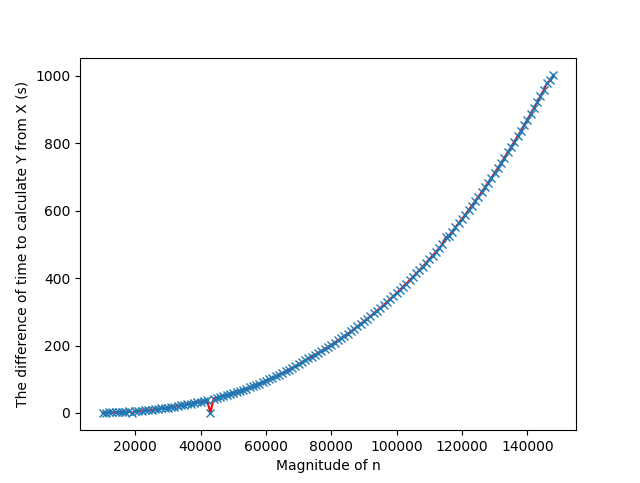
\includegraphics[width=12cm]{n_xy-time_relationship}
\centering
\caption{The relationship between the magnitude of $n$ and the difference of time required to calculate $X$ from $Y$ 
and $X$ using a \textit{brute-force} $X$ calculation algorithm.}
\label{fig:n-xy-time}
\end{figure}

\section{The RSA cipher}
\paragraph*{}
The RSA cipher is by far the most widespread public-key cipher today. Similarly to the Diffie-Hellman key exchange it 
has a public and a private component. However, unlike the Diffie-Hellman key exchange it does not merely solve the 
issue of key distribution. The RSA cipher is a one way permutation, whereas the Diffie-Hellman key exchange distributes
 keys.

\subsection{Method}
\paragraph*{}
The \textit{RSA cipher} operates as follows. The enciphering key is $(e, n)$, where $e$ and $n$ are positive integers. 
The deciphering key is a pair of positive integers $(d, n)$. The enciphering key is made public by all users, while the
 deciphering key is kept secret. Enciphering is done by raising the message to the power of $e$, modulus $n$. 
Deciphering is done by raising the ciphertext to the power $d$, modulus $n$.
$$E(M) \equiv M^{e} \mod n$$
$$D(C) \equiv C^{d} \mod n$$

\paragraph*{}
The enciphering keys are chosen as follows.
$$n = p \cdot q$$
where $p$ and $q$ are extremely large, random primes. $n$ must be greater than the numerical representation of $M$. 
When $n$ is made public, it is computationally difficult to discover $p$ and $q$, as factorization of $n$ is 
enormously difficult. The integer $d$ is picked to be a large, random integer which satisfies the following:
$$gcd(d, (p - 1) \cdot (q - 1)) = 1$$
ie. it is relatively prime to $(p - 1) \cdot (q - 1)$. $e$ is computed from $p$, $q$ and $d$, as such:
$$e \cdot d \equiv 1 \mod (p-1) \cdot (q-1)$$

\paragraph*{}
The proof why this method satisfies (\ref{pk-encipher}) and (\ref{pk-decipher}) is given in the following section.

\subsection{Proof}
\paragraph*{}
The proof for why this cipher satisfies both (\ref{pk-encipher}) and (\ref{pk-decipher}) relies on the 
\textit{Euler-Fermat totient theorem}:
\begin{equation} \label{euler-fermat-totient}
M^{\phi (n)} \equiv 1 \mod n
\end{equation}
where $\phi(n)$ is the \textit{Euler totient function}. The \textit{Euler totient function} gives the number of 
positive integers less than $n$ which are relatively prime to it. For prime numbers this is always $n-1$ (as they are 
only divisible by 1 and themselves). Due to the multiplicative property of the \textit{Euler totient function}
\footnote{The multiplicative property of the \textit{Euler totient function} $\phi(ab) = \phi(a)\phi(b)$ is proved by 
the following: Let $A$, $B$ and $C$ be sets of nonnegative integers, which are relatively prime to $a$, $b$ and $ab$, 
respectivelly, then there is a bijection mapping between $A \times B$ and $C$, trivially provable by the 
\textit{Chinese remainder theorem}.}, if $n = p \cdot q$ and $p$ and $q$ are prime:
%TODO Actually prove this
\begin{equation}
\begin{split}
\phi (n) & = \phi (p) \cdot \phi (q) \\
		 & = (p - 1) \cdot (q - 1) \\
		 & = pq - (p + q) + 1 \\
		 & = n - (p + q) + 1
\end{split}
\end{equation}
Since $d$ was chosen to be relatively prime to $(p - 1) \cdot (q - 1)$, ie. to $\phi (n)$, it does, indeed, have a 
multiplicative inverse in the finite field of modulo $\phi (n)$:
\begin{equation} \label{ed-equiv-mod-phi}
e \cdot d \equiv 1 \mod \phi(n)
\end{equation}

\paragraph*{}
Based on the previous deductions, the following can be asserted for the enciphering and deciphering functions $E$ and 
$D$.
$$E(D(M)) \equiv D(M)^{e} \mod n \equiv M^{d^{e}} \mod n \Longleftrightarrow M^{e \cdot d} \mod n$$
and
$$D(E(M)) \equiv E(M)^{d} \mod n \equiv M^{e^{d}} \mod n \Longleftrightarrow M^{e \cdot d} \mod n$$
From equation \ref{ed-equiv-mod-phi}, the following holds:
$$M^{e \cdot d} \equiv M^{k \cdot \phi (n) + 1} \mod n\text{, for a positive integer $k$}$$
According to equation \ref{euler-fermat-totient}:
$$M^{\phi (p)} \equiv 1 \mod p \Longleftrightarrow M^{p - 1} \equiv 1 \mod p$$
Because $p - 1$ divides $\phi (n)$:
$$M^{k \cdot \phi (n) + 1} \equiv M \mod p$$
Similary, for $q$:
$$M^{k \cdot \phi (n) + 1} \equiv M \mod q$$
Finally, due the multiplicative property of the modulus:
$$M^{e \cdot d} \equiv M^{k \cdot \phi (n) + 1} \equiv M \mod n$$

For any positive integer $M$ up to $n$, the previous statement, therefore, implies that $E$ and $D$ are inverse 
functions, therefore achieving the goal of being ciphers.

\subsection{Cryptographic security}
\paragraph*{}
The cryptographic security of this cipher lies in the fact that up to date, no algorithm exists for factoring $n$ with 
the same efficency as enciphering the message. Precisely, the fastest \textit{non-quantum} algorithm for factorizing 
$n$ can do so in the following number of instructions:
$$O(n) = n^{\sqrt{\frac{ln(ln(n))}{ln(n)}}}$$

\paragraph*{}
A simulation has been run for calculating $p$, $q$, $n$, $d$ and $e$ and factorizing $n$ and is presented in figure
 \ref{fig:rsa_sim}\footnote{The code for this simulation is published at 
\url{https://github.com/markovejnovic/Cripto-IA}, as well.}.
\begin{figure}[ht]
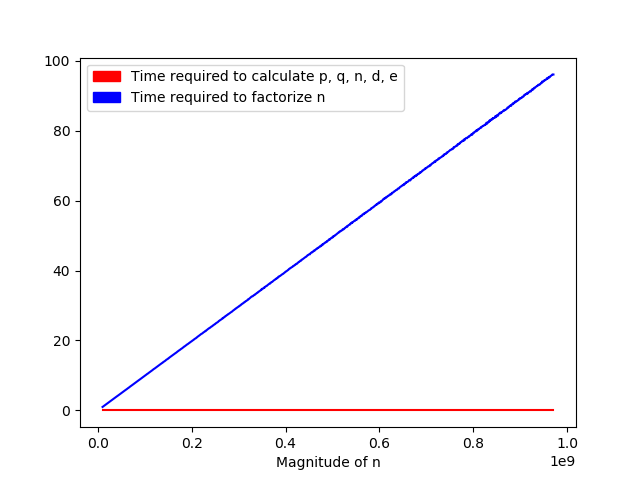
\includegraphics[width=12cm]{rsa_sim}
\centering
\caption{The relationship between the magnitude of $n$ and the time required to calculate $p$, $q$, $n$, $d$ and $e$ 
and factorizing $n$.}
\label{fig:rsa_sim}
\end{figure}

\section{Quantum computers} \label{quantum-comps}
\paragraph*{}
A quantum computer is a computer whose state is described by a point in a $2^{n}$-dimensional vector space, where $n$ 
is the number of individual components\footnote{Although a quantum computer is far more complex than a classical 
computer, I will not be going into the details of the physical phenomena, as that is outside of the scope of this 
paper.}.

\paragraph*{}
The equivalent of the bit\footnote{The basic unit of information which has only 1 state at a time}, in quantum 
computing is the \textit{qubit}. The qubit is able to be in infinite states at the same time, unlike its classical 
counterpart. Due to quantum phenomena, it is able to be in a \textit{superposition}. Upon physical observation of the 
qubit, it collapses into one state. Using \textit{quantum gates}, it is possible to modify the probability of a qubit 
to collapse into a certain state. A qubit is represented using the \textit{ket}-section of the \textit{Dirac notation}:
$$\ket{01}$$
However, when working with the probabilities of a qubit collapsing into a certain state, it is convenient to work with 
vectors:
$$\ket{01} =
\begin{bmatrix}
0 \\
1 \\
0 \\
0 \\
\end{bmatrix}$$
It is helpful to visualize the state of the qubit as a point on an $2^{n}$-dimensional complex unit sphere.

\paragraph*{}
The equivalent of logic gates which convert certain bits to others is the \textit{quantum logic gate}. It is most often
 represented as a matrix which transforms the qubit vector. As an example, the \textit{Pauli X Gate} is presented
\footnote{The \textit{Pauli X Gate} is a gate which does a $\pi$ rotation around the $X$ axis.}:
$$
\begin{bmatrix}
0 & 1 \\
1 & 0 \\
\end{bmatrix}
\begin{bmatrix}
0 \\
1 \\
\end{bmatrix}
=
\begin{bmatrix}
1 \\
0 \\
\end{bmatrix}
$$

\paragraph*{}
This example, however, does not convey the ability of quantum computers. Without the \textit{Hadamard} gate, it is 
imossible to achieve \textit{superpositions}. When \textit{superpositions} are achieved, the probabilistic nature of 
the quantum computer is revealed:
$$
\frac{1}{\sqrt{2}}
\begin{bmatrix}
1 &  1 \\
1 & -1 \\
\end{bmatrix}
\begin{bmatrix}
0 \\
1 \\
\end{bmatrix}
=
\frac{1}{\sqrt{2}}
\begin{bmatrix}
 1 \\
-1 \\
\end{bmatrix}
=
\begin{bmatrix}
 \frac{1}{\sqrt{2}} \\
-\frac{1}{\sqrt{2}} \\
\end{bmatrix}
$$

The probabilities of the qubit collapsing into state $1$ or state $0$ are equal to the square values of the values in 
the vector, therefore, the probability of the qubit collapsing into $1$ is $\frac{1}{2}$, and it is the same for 
collapsing into $0$. The values in the vectors in reality symbolize the lengths of the components parallel to the 
unit vectors, for a vector of length $1$.

\section{Shor's algorithm}
\paragraph*{}
It is because of quantum computers, that the goal of factoring integers in polynomial time has been achieved. In 1195, 
Peter W. Shor, showed that it is, indeed, possible to factorize integers in an extremely small amount of time. This 
algorithm alone, completely negates the possibility of using prime numbers as bases for ciphers.

\subsection{Method}
\paragraph*{}
\textit{Shor's algorithm} operates in two parts: a part preferably achieved on classical computers and a part achieved 
on quantum computers.

\subsubsection{The classical part}
\paragraph*{}
Suppose that $N$ is the composite number, composited from two unknown prime numbers $p$ and $q$. The computer picks a 
random number $a$. Next, the $gcd(a, N)$ is computed. If $gcd(a, N) \not = 1$, then it follows that $a$ is not prime, 
therefore, the algorithm is finished.

\paragraph*{}
Instead of trying to ``\textit{brute-force}'' the prime numbers, \textit{Shor's algorithm} computes the period of 
$a \mod N$, $r$:
\begin{equation} \label{period-shor}
a^r \equiv 1 \mod N
\end{equation}
From the period, which is computed as described in section \ref{quantum-shor}, it is possible to compute one of the 
factors as proven by the following syllogisms.

\paragraph*{}
According to statement \ref{period-shor}, and if one supposes that $r$ is even:
$$N | a^r - 1 \Rightarrow N | (a^{\frac{r}{2}} - 1) (a^{\frac{r}{2}} + 1)$$
With a correct value of $a$, an even value of $r$ can be achieved. Since $r$ is the smallest number for which 
$$N | a^r - 1 \Rightarrow N \nmid a^{\frac{r}{2}} - 1$$
Finally, if $N \nmid a^{\frac{r}{2}}$:
\begin{equation}
\begin{split}
N \nmid a^{\frac{r}{2}} + 1 & \Rightarrow p | a^{\frac{r}{2}} - 1 \\
                            & \Rightarrow q | a^{\frac{r}{2}} + 1
\end{split}
\end{equation}
Since $p$ and $q$ are primes, then:
$$p = gcd(a^{\frac{r}{2}} - 1, N)$$
$$q = gcd(a^{\frac{r}{2}} + 1, N)$$

\subsubsection{The quantum part} \label{quantum-shor}
The first step to calculating the period of is calculating a value $s$ according to the following:
$$2^{s}, n^2 \leq s \leq 2n^2$$
This is required for the further initializing of the quantum states. Notice that $s$ is beetween the squares of $n$. 
This is so, because, as section \ref{quantum-comps} outlines, the probabilities of the collapsed states are squares 
themselves. Next, the registers\footnote{The physical devices which encapsulate \textit{qubits}}, are initialized to 
the following state (each \textit{ket} is a register):
$$\frac{1}{\sqrt{s}} \sum_{b = 0}^{s - 1} \ket{b} \ket{0}$$
Next, $x^b \mod N$ is using repeated squaring\footnote{Repeated squaring is a method often employed to reduce the time 
required to compute a power. It is in essence: $x^n = (x^2)^\frac{n}{2}$ for even numbers and 
$x^n = x(x^2)^\frac{n-1}{2}$ for odd numbers.}
At this point, the registers are in a superposition of:
$$\frac{1}{\sqrt{s}} \sum_{b = 0}^{s - 1} \ket{b} \ket{x^b \mod N}$$
Next, a \textit{quantum fourier transform}\footnote{A \textit{quantum fourier transform}, analogously to a classical 
\textit{Fourier transform} changes the domain, showing where resonance has ocurred the most. \textit{Shor} proposed 
the following method of computing \textit{quantum fourier transformations}. An integer is represented in binary as 
$\ket{a_{l-1} \ket{a_{l-2}} ... a_2 a_1 a_0}$. Suppose two matrices as such exist:
$$R_j =
\begin{bmatrix}
\frac{1}{\sqrt{2}} & \frac{1}{\sqrt{2}} \\
\frac{1}{\sqrt{2}} & - \frac{1}{\sqrt{2}}
\end{bmatrix}$$
and
$$S_j, k = 
\begin{bmatrix}
1 & 0 & 0 & 0 \\
0 & 1 & 0 & 0 \\
0 & 0 & 1 & 0 \\
0 & 0 & 0 & e^{i\frac{\pi}{2^{k - j}}}
\end{bmatrix}$$
$R_j$ operates on a single qubit at index $j$, whereas, $S_j$ operates on \textit{qubits} at positions $j$ and $k$.
These matrices are applied in the following order to the vector prepared for a \textit{Quantum Fourier transformation}:
$$R_{l-1} S_{l-2, l-1} R_{l_2} S_{l-3, l-1} S_{l-3, l-2} R_{l-3} ... S_{0, l-1} S_{0, l-2} ... S_{0, 2} S_{0, 1} R_0$$
} is applied on the first qubit, giving:
$$\frac{1}{\sqrt{s}} \sum_{c = 0}^{s - 1} exp(\frac{2 \pi i bc}{s}) \ket{c}$$
The two registers now are:
$$\frac{1}{s} \sum_{b = 0}^{s - 1} \sum_{c = 0}^{s - 1} exp \left(\frac{2 \pi i bc}{s} \right) \ket{c} \ket{x^b \mod N}
$$

\paragraph*{}
The machine is now observed. The probability of reaching the state $\ket{c, x^k \mod N}$, where $k$ is less than $r$ 
is, as outlined in section \ref{quantum-comps}:
$$\left| \frac{1}{s} \sum exp \left( \frac{2 \pi i b c}{q} \right) \right|^2$$
with the sum being dependent on $a$, over the interval $[0, s)$, such that $x^b \equiv x^k \mod N$, ie. this sum will 
be over all $b$, such that $b \equiv k \mod N$. Now, if one writes $b$ as $dr + k$, the probability is:
$$\left| \frac{1}{s} \sum_{d=0}^{\frac{q - k - 1}{r}} exp \left(\frac{2 \pi i (dr + k) c}{q} \right) \right|^2$$
Let us now define $e$ as $e \equiv rc \mod s$ in the range of $-\frac{s}{2} < e < \leq \frac{s}{2}$. The probability 
is:
$$\left| \frac{1}{s} \sum_{d=0}^{\frac{q - k - 1}{r}} exp \left(\frac{2 \pi i d e c}{q} \right) \right|^2$$
The previous statement is also based on the fact that $exp(\frac{2 \pi i k c}{s}) = 1$ and is therefore factored out.

\paragraph*{}
For this method to be proven viable, it is necessary to prove that when $e$ is small, the amplitudes in this sum go in 
the same direction, so that constructive interference can occur, making the sum amplitude great. Shor proposed 
expressing this sum as an integral:
$$\frac{1}{s} \int_{0}^{\frac{s - k - 1}{r}} exp \left(\frac{2 \pi i d e c}{s} \right) dd + O \left(\frac{s - k - 1}{r} 
\left(exp \left(\frac{2 \pi i e}{s} \right) - 1 \right) \right)$$
The error term is bounded by $O(\frac{1}{s})$ (recall that $|e| \leq \frac{r}{2}$ and that $e^{i \pi} = -1$). Let us 
define $u = \frac{rd}{s}$. Substituting it into the previous integral:
$$\frac{1}{r} \int_{0}^{\frac{r}{s} \frac{s - k - 1}{r}} exp \left(2 \pi i\frac{e}{r} u \right) du$$
If the integral's upper limit is approximated by 1, the resulting error is only, as previously mentioned, 
$O(\frac{1}{s})$:
\begin{equation} \label{prob-int}
\frac{1}{r} \int_{0}^{1} exp \left(2 \pi i\frac{e}{r} u \right) du
\end{equation}
When $|\frac{e}{r}| = \frac{1}{2}$, the equation \ref{prob-int} is:
$$\frac{1}{r} \int_{0}^{1} e^{i \pi u} du = \frac{2i}{\pi r}$$
whose absolute value is:
$$\frac{2}{\pi r}$$
The square of this value ($\frac{4}{\pi^2 r^2}$) is the lower bound of the probability of finding a state 
$\ket{c, x^k \mod N}$. This value is the asymptote under which the probability is. For a sufficiently large $n$, it 
follows that the probability is
$$\frac{1}{3}r^2$$
or greater. This proves sufficient probability of finding the value $r$.

\section{A cipher uncrackable by Shor's algorithm}
\paragraph*{}
Here I present a simple cipher which could potentially resolve the issues presented by the ability of Shor's algorithm 
to find prime numbers. It is in essence, an adapted version of the RSA cipher.

\paragraph*{}
Create vectors $p$ and $q$ of a length $l$ which consists of big positive prime integers as such:
$$p = 
\begin{bmatrix}
p_1 \\
p_2 \\
p_3 \\
\vdots \\
p_l
\end{bmatrix}
q = 
\begin{bmatrix}
q_1 \\
q_2 \\
q_3 \\
\vdots \\
q_l
\end{bmatrix}
$$

Compute their dot product $N = p \cdot q$.
Compute the number $d$ such that:
$$d = gcd(|p| \mod N,\phi(N))$$

Finally, compute $e$, such that
$$e \cdot d \equiv 1 \mod \phi(N)$$

\paragraph*{}
The advantage of this cipher is that it is unfactorable by Shor's algorithm. As Shor's algorithm searches for the 
period of a finite field, and only $N$ is revealed to the public space, and as $N$ is the dot product of the 
individual factors, it is theoretically impossible to find the period of the individual terms of the individual 
vectors. It is, of course, still possible, to \textit{brute-force} calculate the individual vectors, but for so many 
values it is computationally slow. This, algorithm, does require further peer-reviewal and potential improvements.

\paragraph*{}
Another method for creating ciphers which are unbreakable by Shor's algorithm is by incorporating complex analysis, ie.
 the Fourier transformation in the enciphering section, therefore, disabling further possibility of analyzing periods. 
However, I did not manage to achieve this in the scope of this paper.

\section{Conclusion}
\paragraph*{}
Modern criptography focuses on the infeasability of cracking ciphers in a reasonable amount of time, rather, than 
secrecy. The Diffie-Hellman key exchange and the RSA cipher are only some of the most promiment examples of ciphers.
With the advent of quantum computers, the strength of these ciphers is put to question. Shor's algorithm allows for 
factorizing numbers, which is what most public-key ciphers are based on. Even discrete logarithms are solvable using 
quantum computers (Shor, Peter W.). I do believe that, however, it is possible to create public-key ciphers which 
aren't crackable by quantum computers. I believe that the solution for these is using methods which obfuscate the 
periodic nature of finite fields, as described in the previous section.

\pagebreak
\section*{Works cited}
\begin{hangparas}{.25in}{1}
\textit{A Brief History of Cryptography}. http://cryptozine.blogspot.com/2008/05/brief-history-of-cryptography.html

Diffie, W., and M. Hellman. ``\textit{New Directions in Cryptography.}'' IEEE Transactions on Information Theory, vol. 22, no. 6, 1976, pp. 644–654., doi:10.1109/tit.1976.1055638.

Hunter, J. D. \textit{Matplotlib: A 2D graphics environment}. Computing In Science \& Engineering, vol. 9, no. 3, 2007, pp. 90-95., doi:10.1109/MCSE.2007.55

Gauss, Carl Friedrich. \textit{Disquisitiones Arithmeticae}. Yale University, 1966.

International Organization for Standardization. ``\textit{ISO 7498-2:1989.}'' ISO 7498-2:1989, International Organization for Standardization, www.iso.org/standard/14256.html.

Leeuwen, J. van. \textit{Handbook Of Theoretical Computer Science}. Elsevier Science Publishers, 1990, p. 719.

Python Software Foundation. \textit{Python Language Reference}, version 2.7. Available at \url{http://www.python.org}

Rivest, R. L. et al. ``\textit{A Method For Obtaining Digital Signatures And Public-Key Cryptosystems}''. 1977, Accessed 27 Mar 2018.

Sawer, Patrick. ``\textit{The Unsung Genius Who Secured Britain's Computer Defences and Paved the Way for Safe Online Shopping.}'' The Telegraph, 11 Mar. 2016.

Schneier, Bruce. \textit{Applied Cryptography, Second Edition: Protocols, Algorthms, And Source Code In C}. 2nd ed., John Wiley \& Sons, Inc., 1996.

Shor, Peter W. ``\textit{Polynomial-Time Algorithms for Prime Factorization and Discrete Logarithms on a Quantum Computer.}'' SIAM Journal on Computing, 1994, doi:10.1137/S0097539795293172.

\textit{sshd\_config(5) Linux User's Manual}. 2006.

Ylonen, T. \textit{The Secure Shell (SSH) Protocol Architecture}. Internet Requests for Comments. Edited by Lonvick, C. The Internet Society, 2006.
\end{hangparas}
\end{document}
